\documentclass[12pt, a4paper]{article}
\usepackage[utf8]{inputenc}
\usepackage[T1]{fontenc}
\usepackage{fullpage}
\usepackage{hyperref}
\usepackage[parfill]{parskip}
\usepackage{natbib}
\usepackage{url}
\usepackage{amsmath}
\usepackage{graphicx}
\graphicspath{{images/}}
\usepackage{vmargin}
\usepackage[nottoc,numbib]{tocbibind}
\usepackage[strings]{underscore}


\title{Lab Assignment 2: Where’s Croc}	% Title
\author{André Le Blanc, Joel Wallin}
\date{\today}			

\makeatletter
\let\thetitle\@title
\let\theauthor\@author
\let\thedate\@date
\makeatother

%----------------------------------
% Wizard stuff
%----------------------------------
\newcommand{\HMM}[0]{%
  \mathtt{HMM}
}

\begin{document}

\begin{titlepage}
	\centering
    \vspace*{0.5 cm}
    %\includegraphics[width=5cm,height=5cm,keepaspectratio]{deadrop_text.png}\\[0.5 cm]
    %\includegraphics[width=5cm,height=5cm,keepaspectratio]{deadrop_logo.png}\\[1 cm]
    %\textsc{\huge Artificial Intelligence (1DL340) fall 2016}\\[2.0 cm]
	%\textsc{\Large \today}\\[0.5 cm]
	\rule{\linewidth}{0.2 mm} \\[0.4 cm]
	{ \huge \bfseries \thetitle}\\  
	\rule{\linewidth}{0.2 mm} \\[1.5 cm]
    \includegraphics[width=10cm,height=10cm,keepaspectratio]{crocD.jpg}\\[0.5 cm]
    
    \textsc{\Large Lab Group 14:}\\[0.5 cm]
	\begin{minipage}{0.4\textwidth}  
    \begin{align*}
	&\text{André Le Blanc}    &&\text{910930-3850}\\
	&\text{Joel Wallin}  &&\text{941123-3134}\\
	\end{align*}
	\end{minipage}\\[2 cm]
\end{titlepage}


\newpage
\tableofcontents
\newpage

\section{Introduction}

In this lab assignment the task was to guide a park ranger to a crocodile. The crocodile can hide in any of forty water holes in the area and it is unknown which one it is at. In order to find out if the crocodile is in a specific waterhole the park ranger has to search that particular waterhole. The crocodile also moves between the water holes, meaning that the crocodile could be in a waterhole that we have searched previously. Luckily there is information about the average value and standard deviation of salinity, nitrogen and phosphate in every water hole. The crocodile is also equipped with a sensor which at every step in the program has the current measured value of salinity, nitrogen and phosphate. With this information a hidden Markov model and the forward algorithm is used to assign every waterhole a probability that the crocodile is there.

\subsection{Tools used for the project}

The program is written in R, a high level multiparadigm language designed for statistical computing. RStudio is used as the development environment and Git\cite{git} for version control. 

\section{Algorithms}

Evaluating the probability that the crocodile is at a given waterhole (node) is done with the help of a hidden Markov model ($\HMM$)\cite{hmm}. And the forward algorithm\cite{falg} is used to predict at which node it is most likely that the crocodile is. But in order to do that accurately, the $\HMM$ has to take the nature of the problem space into account.

\subsection{Hidden Markov models}

Markov chains are a tool to represent a problem of both discrete and continuous state space. It can be described as a memoryless stochastic process which satisfies the Markov property. Which says that the probability distribution of future states only depends on the present state, it does not care about prior events, i.e. the state at time $t+1$ only depends on state at time $t$. For a discrete problem space, a state's transition probabilities to other states and itself must sum up to 1, as there will always be a transition at every time interval (even if it is just to itself)\cite{hmm}\cite{MA-hmm}. Consider a simple example with two states, rain and sun. If it is raining today, the chance that it rains tomorrow is 40\%. And if it is sunny today, the chance that it will be sunny tomorrow is 30\%. This is represented in figure \ref{fig:rain-sun}.

\newpage
\begin{figure}[!ht]
\centering
\includegraphics[width=8cm,height=4cm,keepaspectratio]{imgs/rainy_sunny.png}\\
\caption{The rings represent states, the arrows transitions and the numbers the transition probabilities.}
\label{fig:rain-sun}
\end{figure}

This system can also be represented as a matrix in matrix \ref{eq:matrix}, with the first row for rain's transition probabilities and the second for the sun's.

\begin{equation}\label{eq:matrix}
\begin{bmatrix}
       0.4 & 0.6\\
       0.3 & 0.7
\end{bmatrix}
\end{equation}

$\HMM$s are used to represent probability distributions of both discrete and continuous problem space through a sequence of observations which relate to the process' state. Lets only consider a discrete number of states. With a Markov chain for all transitions in the system (called the transition matrix), the observations can be used to weight the probability of states in the system. These observations are called  emission probabilities and can be represented as a Markov chain if there are a discrete number of values\cite{hmm}\cite{MA-hmm}. Continuing with the rain and sun example, an observation might be that if a person is wearing a raincoat it is more likely that is raining. So the probability that it is raining will be increased.

Unlike Markov chains, the state is not directly visible in a $\HMM$, but the output is. In $\HMM$ 'hidden' means that it is the state sequence which is unknown, not necessarily the parameters. So an $\HMM$ assumes that each observation is generated by some unknown process which state is hidden. This hidden process is also independent of all prior states. This means that the current state encapsulates all the history needed to predict the future of the process\cite{hmm}\cite{MA-hmm}.

%Lets say we have two urns called gray and blue. Both urns contain 10 marbles. 8 of the marbles in urn gray are white and 2 are black. In urn blue we have 8 black marbles and two white marbles. Let the urns represent two states in a Markov chain and when we are at a state we take a marble and record what color the marble is before putting it back. If we can't see what urn (state) we are at but we can see what color the chosen marbles are we have a hidden Markov model.

\subsection{Forward algorithm}

The forward algorithm is used in conjunction with a $\HMM$ to calculate the probability of a future state given the information provided from the $\HMM$. The transition probabilities are defined and observations are used to weight the probability of every state.  

Let $S_{i,t}$ represent the state $i$ at time $t$ with $N$ possible states, and $O_t$ the observation at time $t$. In equation \ref{eq:forward} $f(S_{i,t})$ is the probability of $S_{i,t}$\cite{MA-forw}.
\begin{equation}\label{eq:forward}
f(S_{i,t}) = \sum_{k=1}^{N} [f(S_{k,t-1})P(S_{i,t}|S_{k,t-1})]P(O_t|S_{i,t})
\end{equation}
What equation \ref{eq:forward} says is to take the probability of its neighboring transition states in the previous time step, and multiply that by the transition probability that it will transition to its state. Where the initial state has to be defined before the forward algorithm can be used. Once those probabilities have been summed up, that sum is multiplied by the probability that the observation predicts that state. This is done for every state in the system.

Continuing on with the rain and sun example an observation is added, where if it is windy, the probability that it is raining is 80\%. And in the initial state, the two states rain and sun are equally likely. Two iterations of the forward algorithm are calculated in equation \ref{eq:forwardCalc}, with the two observations: windy at t=1 and not windy at t=2. The results for every iteration were normalized to get the probability for the two states. According to the calculation, it is more likely to rain on the first day and be sunny on the second day.
\begin{equation}\label{eq:forwardCalc}
\begin{split}
f(S_{rain,1}) = (1*0.4+1*0.3)*0.8 = 0.56 \mapsto 0.68\hspace{29pt}
\\
f(S_{sun,1}) \hspace{3pt} = (1*0.6+1*0.7)*0.2 = 0.26 \mapsto 0.32\hspace{29pt}
\\
f(S_{rain,2}) \hspace{1pt} = (0.68*0.4+0.32*0.3)*0.2 = 0.07 \mapsto 0.12 \hspace{-1pt}
\\
f(S_{sun,2}) \hspace{4pt} = (0.32*0.6+0.68*0.7)*0.8 = 0.53 \mapsto 0.88\hspace{-1pt}
\end{split}
\end{equation}

%Given a hidden Markov model and information about what the Markov chain has for properties we can calculate the probability that the hidden Markov model is at a certain state by observing the output. Given output $y_{1:t}$ where $y_1$ represents the first output and $y_t$ the last output and the : everything in between. We want to calculate the probability that the Markov chain is at state $x_t$, $P(x_t, y_{1:t})$. 

%We could try to calculate this directly. If we continue the example with urns from the previous section and our first observation is a white ball there is a 80\% chance that we are in urn gray. If the second observation also is a white ball there are two alternatives, either we stayed at state gray and got another white ball or we transitioned to urn blue and got a white ball. If we continued this calculation with more observations we could build a tree with all possibilities. However this tree would be huge if we had many observations. We can use the forward algorithm to calculate the probability with much better time complexity. 

\section{Implementation}\label{sec:implementation}
%A discussion of the hidden Markov model you used, including a discussion of the observable variables you utilized, the parameters of your transition and emission matrices, and your initial state.

For this problem a $\HMM$ has to be developed and refined in order to accurately predict the location of the crocodile. And strategies relating to searching and pathing has to be employed to be able to catch the crocodile. 
% * <ajoel.wallin@gmail.com> 2016-10-14T13:57:21.008Z:
%
% > $\HMM$
%
% ^.

\subsection{Hidden Markov model}

The forty waterholes are represented as nodes with their corresponding number as identifier. Each node has its own row in the transition matrix where the transition probabilities to other nodes are defined. The probability that the crocodile transitions to an edge node is uniformly distributed between all the edge nodes, i.e. all edge nodes have the same probability (including the current one). A lot of the information about the probability distribution of variables was attained through analyzing the code of $ \mathtt{WheresCroc.R}$, including the transition probabilities.

Every node has its mean and standard deviation for salinity, phosphor and nitrogen defined. The crocodile's sensor has readings for the current value of those three variables at the node it is located. The emission probabilities cannot comfortably be represented discretely. Each observation is therefore evaluated in a continuous interval at every node to approximate the probability. It is assumed that the readings at each node has a normal distribution as represented in equation \ref{eq:distribution}.

\begin{equation}\label{eq:distribution}
X \sim N(mean,\sigma)
\end{equation}

The probability that the reading comes from a given node is approximated through the formula in equation \ref{eq:mathemission}, where $n$ is a node, $obs$ is the reading from the crocodile's sensor and $a,b$ are two arbitrary values. This is done for all three variables and the three probabilities calculated for each node are normalized in relation to the probability of all other node. The three normalized probabilities are then multiplied together to get the ultimate probability. Equation \ref{eq:Remission} is equivalent to equation \ref{eq:mathemission} in R code.
% \begin{equation}\label{eq:mathemission}
% \begin{split}
% p(n) = P(obs-\sqrt{\sigma} < X \le obs+\sqrt{\sigma}) \hspace{137pt}
% \\
% =\phi((obs+\sqrt{\sigma}-mean)/\sqrt{\sigma})-\phi((obs-\sqrt{\sigma}-mean)/\sqrt{\sigma})
% \end{split}
% \end{equation}
% \begin{equation}\label{eq:Remission}
% p(n) = pnorm(obs+\sqrt{\sigma},mean,\sigma)-pnorm(obs-\sqrt{\sigma},mean,\sigma)
% \end{equation}
\begin{equation}\label{eq:mathemission}
\begin{split}
p(n) = P(obs-a < X \le obs+b) \hspace{137pt}
\\
=\phi((obs+b-mean)/\sqrt{\sigma})-\phi((obs-a-mean)/\sqrt{\sigma})
\end{split}
\end{equation}
\begin{equation}\label{eq:Remission}
p(n) = pnorm(obs+b,mean,\sigma)-pnorm(obs-a,mean,\sigma)
\end{equation}

This formula corresponds to calculating the area of the probability distribution between the two points $a,b$ on the x-axis. Which is highlighted with blue in figure \ref{fig:normal.png}.

\begin{figure}[!ht]
\centering
\includegraphics[width=10cm,height=10cm,keepaspectratio]{imgs/normal.png}\\
\caption{The area between $a,b$.}
\label{fig:normal.png}
\end{figure}

The status of the tourists are also considered. If a tourist is eaten at a node, that node is given the probability of $1$ and all other nodes the probability of $0$, as the crocodile must be at that node. The forward algorithm is used to find the node with the highest probability, where in the initial state all nodes have the same probability.

\subsection{Path finding}
A modified depth-first search algorithm\cite{dfsearch} is used to find the shortest path to the crocodile's predicted location. The algorithm traverses the graph and is careful not to visit any node twice until it gets to the destination. But it does not stop there (the modified part), it continues to search to find more routes. It also keeps track of the shortest evaluated path and does not search at depths greater than that path. By analyzing the graph it can be determined that there is no path longer than 10. Which means that it is possible to drastically improve the performance of the modified DFS through limiting the depth at which it searches to less or equal to 10. The end result is that the shortest path to a node is found. The ranger goes as far as possible at every step and only stops to search if the predicted node of the crocodile is in range.

%\subsection{Non-$\HMM$ strategies}
%A discussion of additional strategies you made use of to improve your performance, including your route finding algorithm for moving between locations and your choice of locations to move to. Explain why you used these strategies.


\section{Results}

%In order to measure the effectiveness of different heuristics, A* strategies and non A* strategies, hundreds of different runs were executed with different variations of these parameters. Then the different strategies were evaluated by looking at the expected value (the mean in this case) and the standard deviation of their series of results.
In order to measure the effectiveness of different approximations of the emission probabilities and strategies, thousands of runs were executed. The different implementations were compared by their mean and standard deviation enable further experiments and optimization of the solution. 

\subsection{Accuracy of the implementation}
% \begin{equation}\label{eq:RemissionInt}
% p(n) = pnorm(obs+a,mean,\sigma)-pnorm(obs-b,mean,\sigma)
% \end{equation}
To approximate the emission probabilities the approach discussed in section \ref{sec:implementation} was used and experimented with different intervals as described in equation \ref{eq:Remission}. Using smaller values of $a,b$ yielded better performance than using larger values. A dynamic interval was also experimented with, where $a,b$ were set to $\sqrt{\sigma}$ and it was able to remain competitive with the smaller intervals of $a,b$

Once the $a,b$ parameters in equation \ref{eq:Remission} went below $0.5$ there was little to no improvement, and going too low with $>0.05$ lead to worse performance. In figure \ref{fig:box-sqrt-fif.png}, 1,000 runs of the program has been run where the first box plot has $a,b$ set to $\sqrt{\sigma}$ and the second to $0.15$. It is not clear in the figure, but the smaller interval performs slightly better with an average of 4.469 versus 4.597 of the dynamic one. The variance is smaller also with 2.512 versus 2.591.%\newpage

\begin{figure}[!ht]\label{fig:box-sqrt-fif.png}
\centering
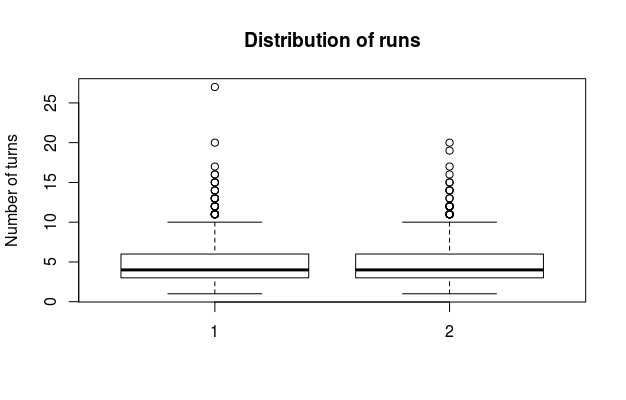
\includegraphics[width=10cm,height=10cm,keepaspectratio]{imgs/box-sqrt-fif.png}\\
\caption{Comparing (1): $\sqrt{\sigma}$, with (2): 0.15}
\end{figure}

Using the static interval for emission probabilities, the accuracy of the whole model and the forward algorithm can be calculated. Doing 1,000 runs, the times that the algorithm predicts the right node is $\sim68.64\%$. With a weighted accuracy, where locality is taken into account as defined in equation \ref{eq:accuracy}, the accuracy is $\sim82.79\%$. The accuracy of every prediction is summed up and divided by the number of predictions to get that result.
\begin{equation}\label{eq:accuracy}
\begin{split}
\mathtt{distance(n_{croc}, n_{prediction})}=d, \; \mathtt{the \; distance \; between \; two \; nodes.}
\\
\mathtt{accuracy(n_{prediction})} = 1 / d, \; \mathtt{if} \; d > 0 \hspace{151pt}
\\
\mathtt{accuracy(n_{prediction})} = 1, \; \mathtt{if} \; d = 0 \hspace{163pt}
\end{split}
\end{equation}

%\subsection{Different path finding algorithms}
%Different path finding algorithms: A*, (Dijkstra), modified DFS.

%The two different path finding algorithms used were the modified DFS described in \ref{sec:implementation} and A*\cite{aStar}. Finding a good heuristic proved to be difficult and there were problems of the algorithm going in circles at times. The average time to calculate the optimal path with both methods took a very long time, however by analyzing the graph it can be determined that there is no path longer than 10. Which means that it is possible to drastically improve the performance of the modified DFS through limiting the depth at which it searches to less or equal to 10.

\subsection{Comparing implementation}

The implementation seems to be performing well, but how does it compare to a random solution which picks nodes at random? In figure \ref{fig:box-fif-random.png} the box plot at index one is the one with $a,b=0.15$ and the second is the random solution. It is extremely clear that the $\HMM$ and forward algorithm improves the performance significantly to a naive random guessing solution.

\begin{figure}[!ht]
\centering
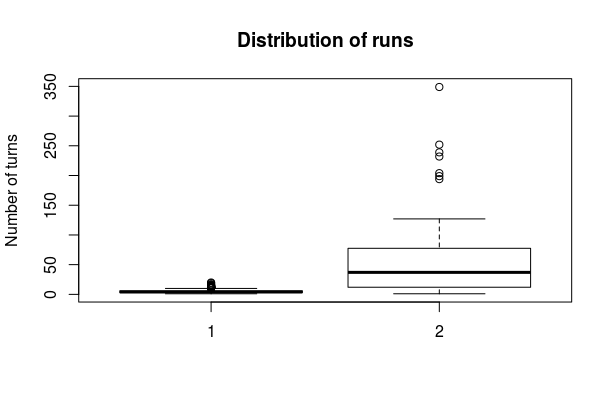
\includegraphics[width=10cm,height=10cm,keepaspectratio]{imgs/box-fif-random.png}\\
\caption{Comparing (1): $a,b=0.15$, with (2): random}
\label{fig:box-fif-random.png}
\end{figure}

\section{Discussion}

The average number of moves in the result clearly speak for themselves. The way the transition and emission probabilities were represented clearly made the forward algorithm undoubtedly effective. There certainly is room for improvement in the approximation of the emission probabilities and other strategies, but the current implementation is still working extremely well.

One area that could be improved are strategies relating to selecting the best route. At the start of the program, the forward algorithm will have less information to go on and be less accurate. To counteract that and minimize the number of unnecessary moves in the beginning, the path algorithm could go towards the middle of the graph during the first couple of moves if the predicted node is not too far away. This fixes a problem where the ranger would sometimes go forwards and backwards in the graph. Another strategy that could be employed is to take routes that cumulatively have higher probability of the crocodile being there, instead of only looking at the node with the highest probability.

Another part of the path finding that could be improved is the algorithm for finding the shortest path. The modified DFS algorithm is quite expensive time complexity wise and could be improved by using Dijkstra's algorithm. But due to sloppy A* code and time constraints it was easier to implement a naive DFS solution instead.

%Also the strategy could be improved, as the first two predictions of the forward algorithm often are wrong. One such strategy would be to during the first two moves, only go to the predicted destination if its within a two move range. Otherwise go towards the middle of the graph, ex. node 25. This minimizes the unnecessary moves that often are done at the beginning of the game.

\section{Conclusion}

%The best parameters for implementing an A* algorithm for this particular problem is to use the Manhattan distance as the heuristic and to slightly penalize high costs between nodes. And running the A* algorithm after every step the delivery man takes. Waiting is generally useless due to the costs of the roads tending to increase as time goes by. Which also favors A* going fairly straight towards the destination. Using graph search is also a better idea than tree search due to the existence of loops.

%The implemented A* algorithm yields a better result than a person stepping through the graph unless the person extensively analyses the grid's state. This is due to the algorithm quickly and accurately finding a cost efficient path to its destination. That said, it is possible to improve the algorithm. As it is somewhat limited in its ability to determine an optimal order for picking up and delivering packages. So a person could still outperform the algorithm by doing time consuming analysis of the grid's state.

The difficult part about implementing a $\HMM$ for this particular problem is calculating the emission probabilities as the transition probabilities are already nicely defined. A good way of doing this is assuming that the readings from each waterhole is normally distributed and use the available means and standard deviations to calculate a probability distribution of the readings being within a small interval. Also utilizing the tourists as absolute observations when they are eaten at a particular node improves the model's performance.

Improvements that can be made to the implementation is the strategy for finding a path to the crocodile. Traversing the shortest path works well in some situations, a better solution would be to take paths that cumulatively are more likely of the crocodile being there and thereby minimizing the number of unnecessary moves that the ranger has to take.

\raggedright
\bibliography{cit.bib}{}
\bibliographystyle{unsrt}

\end{document}
